
\documentclass{article} % For LaTeX2e
\usepackage{iclr2026_conference,times}

% Optional math commands from https://github.com/goodfeli/dlbook_notation.
\input{math_commands.tex}

\usepackage{hyperref}
\usepackage{url}
\usepackage{amsmath}
\usepackage{amssymb}
\usepackage[T1]{fontenc}
\usepackage[pdftex]{graphicx}

\renewcommand{\cite}{\citep}

% \title{Predictability Shapes Adaptation: An Evolutionary Perspective on Modes of Learning in Transformers}
% \title{An evolutionary perspective on strategy \\ preference in Transformers}
\title{An evolutionary perspective on modes of \\ learning in Transformers}

% Authors must not appear in the submitted version. They should be hidden
% as long as the \iclrfinalcopy macro remains commented out below.
% Non-anonymous submissions will be rejected without review.

\author{Alexander Y. Ku$^{1,2}$, Thomas L. Griffiths$^2$, Stephanie C.Y. Chan$^1$ \\
$^1$Google DeepMind\\
$^2$Department of Psychology, Princeton University\\
\texttt{\{alexku, scychan\}@google.com, tomg@princeton.edu}
}


% The \author macro works with any number of authors. There are two commands
% used to separate the names and addresses of multiple authors: \And and \AND.
%
% Using \And between authors leaves it to \LaTeX{} to determine where to break
% the lines. Using \AND forces a linebreak at that point. So, if \LaTeX{}
% puts 3 of 4 authors names on the first line, and the last on the second
% line, try using \AND instead of \And before the third author name.

\newcommand{\fix}{\marginpar{FIX}}
\newcommand{\new}{\marginpar{NEW}}

\iclrfinalcopy % Uncomment for camera-ready version, but NOT for submission.
\begin{document}

\maketitle

\begin{abstract}
The success of Transformers lies in their ability to improve inference through two complementary strategies: the permanent refinement of model parameters via \textit{in-weight learning} (IWL), and the ephemeral modulation of inferences via \textit{in-context learning} (ICL), which leverages contextual information maintained in the model's activations.
Evolutionary biology tells us that the predictability of the environment across timescales predicts the extent to which analogous strategies should be preferred. Genetic \textit{evolution} adapts to stable environmental features by gradually modifying the genotype over generations. Conversely, environmental volatility favors \textit{plasticity}, which enables a single genotype to express different traits within a lifetime, provided there are reliable cues to guide the adaptation.
We operationalize these dimensions (environmental stability and cue reliability) in controlled task settings (sinusoid regression and Omniglot classification) to characterize their influence on learning in Transformers.
We find that stable environments favor IWL, often exhibiting a sharp transition when conditions are static. Conversely, reliable cues favor ICL, particularly when the environment is volatile.
Furthermore, an analysis of learning dynamics reveals task-dependent transitions between strategies (ICL $\to$ IWL and vice versa). We demonstrate that these transitions are governed by (1) the asymptotic optimality of the strategy with respect to the environment, and (2) the optimization cost of acquiring that strategy, which depends on the task structure and the learner's inductive bias.
\end{abstract}

% \begin{abstract}
% Transformer models learn in two distinct modes: in-weights learning (IWL), encoding knowledge into model weights, and in-context learning (ICL), adapting flexibly to context without weight modification.
% To better understand the interplay between these learning modes, we draw inspiration from evolutionary biology's analogous adaptive strategies: genetic encoding (akin to IWL, adapting over generations and fixed within an individual's lifetime) and phenotypic plasticity (akin to ICL, enabling flexible behavioral responses to environmental cues). In evolutionary biology, environmental predictability dictates the balance between these strategies: stability favors genetic encoding, while reliable predictive cues promote phenotypic plasticity.
% We experimentally operationalize these dimensions of predictability and systematically investigate their influence on the ICL/IWL balance in Transformers. Using regression and classification tasks, we show that high environmental stability decisively favors IWL, as predicted, with a sharp transition at maximal stability. Conversely, high cue reliability enhances ICL efficacy, particularly when stability is low. Furthermore, learning dynamics reveal task-contingent temporal evolution: while a canonical ICL-to-IWL shift occurs in some settings (e.g., classification with many classes), we demonstrate that scenarios with easier IWL (e.g., fewer classes) or slower ICL acquisition (e.g., regression) can exhibit an initial IWL phase later yielding to ICL dominance. These findings support a relative-cost hypothesis for explaining these learning mode transitions, establishing predictability as a critical factor governing adaptive strategies in Transformers, and offering novel insights for understanding ICL and guiding training methodologies.
% \end{abstract}

% \begin{abstract}
% Transformer models can learn in two quite different ways: in-weights learning (IWL; encoding knowledge in model weights) vs. in-context learning (ICL; flexibly adapting to context without weight changes). To better understand the balance and dynamics between these two types of learning, we turn to evolutionary biology, which exhibits analogous modes of adaptation: genetic encoding of behavior (akin to IWL; adapting over longer timescales but fixed within the lifetime of an individual) vs. phenotypic plasticity (akin to ICL; where behavior is not hardcoded and instead flexibly adapts to the environment). In evolutionary biology, the balance between these two modes of adaptation depends on environmental predictability; specifically, environmental stability favors genetic encoding, while the reliability of cues in predicting future conditions favors phenotypic plasticity. In this work, we experimentally operationalize these two types of predictability, and systematically investigate how they govern the ICL/IWL balance in Transformers. Using simple regression and classification tasks, we show that high environmental stability strongly promotes IWL over ICL, with a sharp transition to IWL at maximal stability, while high cue reliability enhances ICL efficacy, especially when environmental stability is low. Furthermore, learning dynamics reveal that the time course of ICL and IWL depends on the task: the typical shift from ICL to IWL occurs in some settings (e.g., classification with many classes), but we demonstrate that in settings where IWL is easier (e.g., classification with fewer classes) or when ICL is more slowly acquired (e.g., regression) learning can show an initial IWL phase later ceding to ICL dominance. These findings support a relative-cost hypothesis for shifts between types of learning and establish predictability as a critical factor shaping adaptive learning in Transformers, offering insights for understanding ICL and guiding training methodologies.
% \end{abstract}
\section{Introduction}

Transformers \cite{vaswani2017attention} underpin the success of modern large language models (LLMs), demonstrating impressive performance across a diverse set of tasks \cite{brown2020language}. A key emergent capability of these models is \textit{in-context learning} (ICL), which allows them to perform novel tasks specified by examples in the input prompt, without updating model parameters \cite{brown2020language, dong2022survey, liu2023pre}. This stands in sharp contrast to standard \textit{in-weights learning} (IWL), where knowledge is gradually encoded into the model parameters during training.
Research into the nature of ICL is extensive, ranging from mechanistic accounts including induction heads \cite{olsson2022context} and function vectors \cite{todd2023function}, to theoretical frameworks that interpret ICL as a form of implicit optimization or Bayesian inference \cite{von2023transformers, dai2022can, xie2021explanation}. Most relevant to this work, however, is the finding that the emergence of ICL relies on specific statistical properties of the training data \cite{chan2022data}.

While the emergence of ICL can be productively understood in terms of rational adaptation to environmental pressures \cite{wurgaft2025context}, this perspective has limitations. By focusing on what the asymptotically optimal strategy is (i.e., ICL or IWL), it struggles to account for the learning dynamics, particularly the factors that precipitate transitions between strategies. This gap is significant because empirical studies show that ICL can be transient, emerging early in training only to diminish or be superseded by IWL as the model converges \cite{singh2023transient}.

In this paper, we argue that evolutionary theory offers a powerful explanatory lens for understanding these learning dynamics. Specifically, we examine the environmental factors that drive transitions between two analogous biological strategies: \textit{plasticity} and \textit{evolution}. Plasticity is the capacity of a single genotype to produce different phenotypes (e.g., morphological or behavioral changes) in response to environmental cues. It allows for adaptation within an individual's lifetime, mirroring how ICL modulates inference based on a prompt. Conversely, evolution involves the slow modification of the genotype across generations via selection to produce specific adaptive traits, analogous to updating model parameters via IWL. Furthermore, just as evolution gives rise to plasticity, the capacity for ICL is acquired through the process of IWL.

Evolutionary theory suggests that the reliability of information across timescales determines which adaptive strategy is favored \cite{stearns1989evolutionary}. Plasticity is generally selected for in fluctuating environments, provided reliable cues are available to guide the adaptive response \cite{stearns1989evolutionary, stephens1989variance}. However, plasticity tends to be selected against when the environment is stable enough to obviate the need for flexibility, when reliable cues are unavailable, or when the inherent costs of plasticity are prohibitive \cite{stearns1989evolutionary, stephens1989variance, dewitt1998costs}. Furthermore, \textit{genetic assimilation} describes the evolutionary process by which plastic traits become fixed, eventually rendering their expression insensitive to the cues that originally produced them \cite{waddington1953genetic, pigliucci2006phenotypic}. This phenomenon parallels the empirically observed transience of ICL, where the model's reliance on the prompt diminishes as the task is consolidated into weights \cite{singh2023transient}.

We hypothesize that analogous factors govern the competition between ICL and IWL in Transformers, determining which strategy dominates at different stages of training. To test this, we operationalize two key dimensions: \textit{cue reliability}, defined as the sufficiency of information within a single prompt to specify the target task, and \textit{environmental stability}, defined as the invariance of the target task across different prompts encountered during training. We manipulate these dimensions in two controlled settings: parametric sinusoid regression and few-shot Omniglot classification. Our results confirm that the evolutionary principle regarding environmental predictability across timescales accurately predicts the learning dynamics of Transformers. This suggests that an ecological view of training environments can offer principled guidance for developing new training methodologies.

% Transformers \cite{vaswani2017attention} underpin the success of modern large language models (LLMs), demonstrating impressive performance across diverse tasks \cite{brown2020language}. A key emergent capability of these models is in-context learning (ICL), where models adapt to novel tasks specified by examples given in the input prompt, without requiring gradient-based parameter updates \cite{brown2020language, dong2022survey, liu2023pre}. This rapid and flexible adaptation contrasts with standard in-weights learning (IWL), where knowledge is gradually encoded into model parameters during training \cite{chan2022data, singh2023transient}. The mechanisms enabling ICL are an active area of research, with theories encompassing induction heads that copy and complete patterns \cite{olsson2022context, elhage2021mathematical}, function vector heads that compute task representations \cite{todd2023function, hendel2023context}, and interpretations of ICL as implicit optimization or Bayesian inference within the forward pass \cite{von2023Transformers, dai2022can, xie2021explanation}.

% While IWL traditionally yields stable knowledge from consistent task exposure, the interplay and developmental trajectory between IWL and ICL remain incompletely understood. Notably, ICL capabilities can be transient, emerging early in training but sometimes diminishing or being superseded by IWL as tasks become more predictable or frequently encountered \cite{singh2023transient, anand2024dual}. Characteristics of the data distribution, such as input noise and dynamic input-label mappings --- which influence task predictability --- have also been shown to affect the balance between ICL and IWL \cite{chan2022data, reddy2023mechanistic}. Despite these advances, a comprehensive framework for why and when Transformers shift their reliance between these learning modes is still developing.

% In this paper, we argue that evolutionary biology offers one explanatory lens for understanding this dynamic interplay. Organisms adapt to variable environments via analogous mechanisms: phenotypic plasticity and genetic evolution. Phenotypic plasticity --- the ability of a genotype to produce different phenotypes (e.g., changes in morphology, physiology, or behavior like learning) in response to environmental cues \cite{west2003developmental, scheiner1993genetics} --- allows rapid, within-lifetime adaptation, akin to a Transformer's ICL adapting to a prompt. This contrasts with genetic evolution --- the slower, generational modification of the genotype --- which encodes more permanent traits, analogous to IWL.

% Evolutionary biology has established that environmental predictability critically determines the favored adaptive strategy \cite{stearns1989evolutionary}. Phenotypic plasticity is generally favored when the environment fluctuates and reliable cues are available to guide an appropriate adaptive response \cite{stearns1989evolutionary, stephens1989variance}. However, plasticity may be selected against if the environment is extremely stable (negating the need for flexibility and favoring genetically hardcoded traits), if cues are unreliable, or if the inherent costs of plasticity are too high \cite{stearns1989evolutionary, stephens1989variance, dewitt1998costs}. Furthermore, a key long-term dynamic is genetic assimilation: if an environment that previously favored a plastic response becomes stable, the consistently advantageous phenotype, initially induced plastically by cues, can become genetically encoded, shifting the trait from flexible to fixed \cite{waddington1953genetic, pigliucci2006phenotypic}. This offers a compelling parallel to the observed transience of ICL.

% Building on this evolutionary framework, we hypothesize that analogous dimensions of task predictability govern which modes of learning Transformers adopt and how their balance shifts over time. We operationalize two key dimensions, inspired by these biological concepts: \textit{cue reliability}, defined as the clarity and informativeness of information within a single prompt for specifying the required task, and \textit{environmental stability}, defined as the consistency or predictability of the task structure across different prompts encountered over the course of training. We predict that high environmental stability will favor IWL, while high cue reliability will enhance ICL efficacy, particularly when stability is low. Moreover, we anticipate that conditions of high stability for tasks initially learned via ICL may lead to an ``assimilation'' of these solutions into IWL.

% To test these hypotheses, we employ a controlled experimental design that systematically investigates the independent and interactive effects of cue reliability and environmental stability on the use and development of ICL and IWL. We deploy this approach in two distinct domains: a parametric sinusoid regression task and a few-shot binary classification task on Omniglot images. Our findings aim to establish predictability as a critical factor shaping adaptive learning in Transformers, offering insights for understanding ICL and potentially guiding future training methodologies.

% Transformer architectures \cite{vaswani2017attention} underpin the success of modern large language models (LLMs), demonstrating impressive performance across diverse tasks \cite{brown2020language}. A key emergent capability in these models is in-context learning (ICL), where models adapt to novel tasks specified by examples within the input prompt, without requiring gradient-based parameter updates \cite{brown2020language, dong2022survey, liu2023pre}. This rapid, flexible adaptation contrasts with standard in-weights learning (IWL), where knowledge is gradually encoded into model parameters during training \cite{chan2022data, singh2023transient}. While previous work has begun to elucidate the specific conditions that govern models' preference between ICL and IWL \cite{chan2022data, singh2023transient, bietti_birth_2023, anand2024dual, he2024context, chan_toward_2025, singh_strategy_2025}, this dynamic interplay nonetheless remains incompletely understood.

% In this paper, we argue that one way to understand this interplay is to look to evolutionary biology, where organisms adapt to variable environments via analogous mechanisms. Phenotypic plasticity---the ability of a genotype to produce different phenotypes in response to environmental cues via processes like learning \cite{west2003developmental, pigliucci2001phenotypic}---allows rapid adaptation within a lifetime, akin to ICL adapting to a prompt. For example, certain animals change the thickness and color of their coats in preparation for changing seasons. This phenotypic change is triggered by number of daylight hours, a cue that is predictive of the relevant environmental conditions (temperature and snowfall) \cite{underwood_photoperiod_1980, otte_snow_2024}. This rapid adaptability contrasts with genetic evolution—the slower, generational modification of the genotype—which encodes more permanent traits (analogous to IWL).

% When do organisms evolve to display phenotypic plasticity? Previous research in evolutionary biology has established that it depends critically on the predictability of the environment \cite{scheiner2021loss, leung2020reduced}. Phenotypic plasticity is generally favored when the environment undergoes fluctuations and reliable cues are available to guide an appropriate adaptive response \cite{scheiner2021loss, leung2020reduced}. However, plasticity may be selected against if the environment is either extremely stable (negating the need for flexibility) or if its variations are too erratic and cues too unreliable to permit effective plastic adjustments \cite{leung_reduced_2020, reed2010evolutionary, tufto2015genetic, chevin2015estimating, bonamour2019phenotypic, stamps2020information, lehtonen2021sensitive, king_evolution_2019}.

% Based on this evolutionary framework, we propose that analogous dimensions of task predictability should govern which modes of learning Transformers adopt. We operationalize cue reliability as the clarity and reliability of information within a single prompt for specifying the required task \cite{dall2015learning, lehtonen2021sensitive, stamps2020information} and 
% environmental stability as the stability or predictability of the task across different prompts over time \cite{boyce2006predicting, leung2020evolution}.
% To test the hypothesis that these factors determine what mode of learning Transformers will adopt, we use a controlled experimental design that systematically investigates the independent and interactive effects of cue reliability and environmental stability on the use of ICL and IWL. We deploy this approach in two distinct domains: a parametric sinusoid regression task and a few-shot binary classification task on Omniglot images.

% \section{Approach: Modeling Transformer Learning Dynamics through an Evolutionary Lens}
% \section{Learning dynamics through an evolutionary lens}
\section{Environmental predictability}

Our general approach relies on drawing a correspondence between aspects of biological adaptation and the learning dynamics observed in Transformers. Fundamentally, we view both systems as optimizing for environmental predictability: the strategy selected depends on the timescale at which information is most reliable. To make these parallels concrete, we consider two examples that illustrate the specific phenomena we investigate.

% Our general approach relies on drawing a correspondence between aspects of biological adaptation and the learning dynamics observed in Transformers. Just as ICL and its underlying dynamics are emergent products of IWL, biological plasticity is an emergent property of evolution. To make these parallels concrete, we consider two classic biological examples that illustrate the specific phenomena we investigate in this work.

\textbf{Plasticity.} The classic example of plasticity is the defense adaptation of the water flea, Daphnia \cite{tollrian1999ecology}. When Daphnia detect chemical cues (kairomones) released by predators, they develop a protective helmet and tail spine. In the absence of these cues, individuals with the exact same genotype develop a standard, non-defensive morphology to conserve energy.
Just as the Daphnia phenotype is determined by the interaction of a fixed genotype with an environmental cue, a Transformer’s output is determined by the interaction of fixed weights with the context provided in the prompt. In both cases, the system adapts its behavior to the current environment without modifying its underlying genotype or weights.

\textbf{Genetic assimilation.} The phenomenon where ICL emerges early in training but is later superseded by IWL parallels genetic assimilation, a concept famously demonstrated by Waddington’s selection experiments on Drosophila \cite{waddington1953genetic}. In these experiments, Waddington exposed fruit fly pupae to a heat shock (an environmental cue), which caused a fraction of them to develop a cross-veinless wing structure (a plastic response). By selectively breeding only those individuals that exhibited the trait, he eventually produced a lineage where the cross-veinless trait appeared without the heat shock.
Similarly, a Transformer initially reliant on prompts (ICL) will, given stable training conditions, consolidate the capability into its weights (IWL), rendering the inference insensitive to the contextual cues that originally guided it \cite{singh2023transient}.

At its core, these two phenomena hinge on distinct aspects of environmental predictability: the reliability of cues to guide adaptation within a lifetime, and the stability of the environment to facilitate evolution across generations. Both dimensions ultimately derive from the predictive power of information at different timescales --- specifically, how accurately experience (whether gathered within a single lifetime or accumulated across generations) anticipates optimal behavior. If this correspondence between biological adaptation and learning in Transformers holds, then systematically manipulating predictability at different timescales (e.g., via noise) should allow us to determine the preferred learning strategy in Transformers. The following section details how we operationalize this experimentally in two controlled training environments.

% Our approach leverages analogies between biological adaptation and Transformer learning to investigate the influence of environmental predictability. The core idea is that the emergence, persistence, and transitions between ICL and IWL in Transformers can be understood as parallels to how organisms evolve to use phenotypic plasticity versus genetically determined traits, and how these strategies themselves can shift (e.g., via genetic assimilation).

% To make these parallels concrete:

% \textbf{ICL as Phenotypic Plasticity:} Consider the water flea (Daphnia), which develops protective helmets and spines (phenotype) only when detecting chemical cues from predators (environmental cue) \cite{tollrian1999ecology}. Similarly, many animals adjust coat thickness and color based on changing daylight hours -- a cue predictive of seasonal temperature and snowfall \cite{underwood_photoperiod_1980, otte_snow_2024}. This rapid, reversible, cue-driven adaptation mirrors how a Transformer uses in-context examples (cue) to tailor its output (phenotype) to a novel task without altering its weights (genotype).

% \textbf{IWL as Genetically Determined/Canalized Traits:} The innate, species-specific song of certain songbirds develops reliably, even in acoustic isolation. This exemplifies a genetically underpinned trait that is invariant to environmental variation, a phenomenon known as environmental canalization \cite{marler2014instinct}. Analogously, IWL captures fundamental, consistently useful knowledge (e.g., grammar for an LLM) that is ``hardcoded'' into model weights through sustained exposure to stable patterns.

% \textbf{ICL Transience as Genetic Assimilation:} Waddington's classic experiments showed that a heat-shock-induced crossveinless wing phenotype in Drosophila (a plastic response), after generations of selection, became genetically assimilated, appearing even without the heat shock \cite{waddington1953genetic}. Analogously, if a Transformer initially uses ICL for a task type that later becomes a stable and frequent part of training, the model might ``assimilate'' this solution into its weights (IWL), potentially reducing reliance on ICL for that specific pattern.

% Guided by this framework, particularly the established role of environmental stability and cue reliability in shaping biological adaptation, our experimental design systematically manipulates these two factors within the training regime of Transformers.
% For cue reliability, we vary the clarity or consistency of the in-context examples provided within each prompt.
% % For instance, in the Omniglot classification task, this involves manipulating the consistency of label-to-image pairings in the few-shot examples. In the sinusoid regression task, it could involve varying the noise or number of example points defining the target function within a prompt.
% For environmental stability, we manipulate the consistency of the underlying task rule across successive training batches. 
% % In the classification task, a stable environment might always present the same underlying (but initially unknown) mapping of image classes to target labels across many prompts, while an unstable environment would change this mapping frequently. For regression, stability refers to how consistently the parameters of the target sinusoid function (e.g., phase, amplitude) are drawn from the same distribution or remain fixed across prompts.

% \section{Background and Related Work}

% \stephanie{Given that we need to save space, I think we could cut this  Related Work section, and move the most important refs/content to the intro. It is partially redundant with the intro, as is.}

% \subsection{In-Context Learning vs. In-Weights Learning}

% \stephanie{we might need to cut this subsection completely}

% In-context learning (ICL) is a key emergent capability of Transformers \cite{vaswani2017attention}, referring to their ability to adapt to novel tasks specified by examples within an input prompt, without requiring gradient-based parameter updates \cite{brown2020language, dong2022survey, liu2023pre}. The mechanisms proposed to underpin ICL are diverse. Prominent theories include the role of induction heads, which copy and complete patterns from the context \cite{olsson2022context, elhage2021mathematical, akyurek2024higher, wang2024Transformers}, and the more recently identified function vector (FV) heads, which learn to compute and apply compact task representations \cite{todd2023function, hendel2023context, le2024disentangling}. Other interpretations frame ICL as an implicit optimization process (e.g., akin to gradient descent) performed within the forward pass \cite{von2023Transformers, dai2022can, akyurek2022learning, ding2023Transformer}, or as a form of implicit Bayesian inference \cite{xie2021explanation, wang2023Transformers, prystawski2023think, zhang2024trained, li2023Transformers}. The training regimen that gives rise to ICL is often conceptualized as a meta-learning process, effectively learning an inference-time learning algorithm \cite{finkbeiner2024chip, kirsch2022general, melo2022Transformers, wang2024Transformers}.

% Conversely, in-weights learning (IWL) describes the conventional knowledge acquisition process in neural networks. Here, task-relevant information is gradually encoded into the model's parameters via gradient-based optimization during training \cite{sun_learning_2024, ruis_procedural_2024, zucchet_how_2025}. IWL typically yields more stable and generalized knowledge for tasks that are frequently encountered or possess a consistent structure. A central aim of our research is to understand how the balance and developmental trajectory of these two learning modes are shaped by the statistical properties of the task environment encountered during training.

% \subsection{Learning Dynamics: Transience, Competition, and Data Influence}

% The preference for ICL vs. IWL is notably dynamic, evolving throughout the training process. A significant observation from recent literature is the phenomenon of ICL transience: ICL capabilities often emerge relatively early in training but may subsequently diminish or be superseded by IWL strategies \cite{singh2023transient}. This shift is particularly evident when tasks are encountered repeatedly or become highly predictable within the training data \cite{anand2024dual, he2024context, park2024understanding}.

% The emergence and relative balance of ICL versus IWL are also influenced by broader characteristics of the data distribution. Factors such as the burstiness of token appearance and Zipfian class distributions, which are typical of natural language, have been shown to affect this balance \cite{chan2022data, reddy2024data}. Most relevant to our current study, input noise and dynamic input-label mappings can impact task predictability and also the balance between ICL and IWL \cite{chan2022data}. Studies investigating these aspects have provided compelling initial evidence that variations in predictability can shift the preference between ICL and IWL.

% Mechanistically, the transition between ICL and IWL is hypothesized to involve both competition and cooperation among neural circuits within the Transformer architecture \cite{singh2023transient, park2024understanding, singh_strategy_2025}. For instance, IWL might predominantly engage parameters within MLP layers, whereas ICL often leverages attention-based circuits, such as induction or FV heads \cite{olsson2022context,todd2023function}. While these distinct pathways might compete for representational capacity or influence, IWL-based structures can also scaffold or facilitate the development of ICL mechanisms.

% \stephanie{(optional) add a small section on predictability in Transformers. E.g. Elmoznino 2024, Goldblum 2024} \alex{I think we should put this in the part in future directions where we suggest that "relative-cost" can be characterized in many ways, including complexity.}

% \subsection{Biological Adaptation: Phenotypic Plasticity and Environmental Predictability}

% Biological organisms have evolved diverse strategies to contend with the challenges posed by variable and uncertain environments. A cornerstone of this adaptability is \emph{phenotypic plasticity}: the capacity of a single genotype to produce a spectrum of different phenotypes—spanning morphology, physiology, and behavior—in direct response to specific environmental cues encountered during an individual's development or lifetime \cite{west2003developmental, pigliucci2001phenotypic, scheiner1993genetics}. This facility allows individuals to tailor their characteristics to local conditions, potentially enhancing survival and reproduction relative to organisms with rigidly fixed phenotypes, particularly in heterogeneous or fluctuating settings. Learning, wherein individuals modify their behavior based on experience to navigate and exploit their surroundings, represents a particularly sophisticated form of such behavioral plasticity \cite{dukas1998evolutionary, snell2019evolution}. Phenotypic plasticity is often contrasted with \emph{environmental canalization}, which is the invariance of phenotypes to environmental variation \cite{waddington_canalization_1942, siegal_waddingtons_2002}.

% The existence and evolutionary trajectory of phenotypic plasticity are intricately linked to several dimensions of environmental predictability:

% \textbf{Environmental Stability.} The degree of environmental variation across generations profoundly influences whether plasticity is favored over more canalized (fixed) strategies \cite{boyce2006predicting, leung2020evolution}. In highly stable environments, where the optimal phenotype seldom changes, natural selection typically favors the evolution of a single, well-adapted fixed phenotype. Maintaining the biological machinery for plasticity in such constant scenarios would likely incur unnecessary costs \cite{dewitt1998costs}.

% \textbf{Cue Reliability.} For plasticity to be adaptive, environmental cues must reliably forecast the selective pressures an organism will face when the corresponding phenotype is expressed \cite{dall2015learning, lehtonen2021sensitive, scheiner2021loss}. If cues are noisy or uninformative, plastic responses may be maladaptive.

% A crucial long-term dynamic in this context is \emph{genetic assimilation}. If an environment that previously favored a plastic response becomes stable for an extended duration, the consistently advantageous phenotype, initially induced by cues, can become genetically encoded. This process results in the phenotype being "constitutively expressed" (i.e., activated even in the absence of the original cue), thereby shifting the trait from a flexible, plastic state to a fixed, genetically determined one \cite{waddington1953genetic, west2003developmental, pigliucci2006genetic}.

% \section{Approach: Tying Learning Dynamics to Evolutionary Phenomena}

% \stephanie{this is also a bit redundant with the intro, and can probably be cut / incorporated into there if needed}

% The rich theoretical framework of evolutionary biology
% % , particularly concerning phenotypic plasticity and its adaptation to environmental predictability,
% offers a potent explanatory lens for understanding the dynamic interplay between ICL and IWL in Transformers. We propose that drawing analogies between these domains can provide computational-level insights \cite{marr82vision} into why specific learning strategies emerge, persist, or transition within these models.

% Our central thesis posits a direct correspondence between these learning modalities and established biological adaptation strategies. ICL strongly mirrors phenotypic plasticity. A classic biological illustration is the development of defensive structures in water fleas (Daphnia). When these organisms detect chemical cues (kairomones) from predators, individuals can develop protective helmets and elongated tail spines, significantly enhancing their survival prospects without any genetic change. In the absence of such cues, they forgo these energetically costly structures \cite{agrawal1999specific_study_if_available, tollrian1999predator_cues_daphnia}. This rapid, cue-driven, and often reversible adaptation is strikingly analogous to how a Transformer, when provided with a few demonstration examples in its context window (the "cue"), tailors its output (the "phenotype") to a novel task---be it translation, sentiment analysis, or code generation---without undergoing retraining, thereby leaving its "genotype" or weights unchanged.

% Conversely, IWL finds its parallel in genetically determined or canalized traits. An example from the natural world is the innate, species-specific song of many songbirds. While some avian species exhibit significant song learning (a form of plasticity), others possess highly stereotyped songs that develop reliably even when individuals are reared in acoustic isolation from conspecifics \cite{marler1991birdsong_innateness_example; e.g., some flycatchers or other species with highly innate songs}. This points to a strong genetic underpinning and developmental canalization, ensuring the consistent structure of the song, which is often vital for species recognition and successful mating. In a similar fashion, IWL captures fundamental, consistently useful knowledge---such as the grammatical rules of a language for an LLM, or core visual features for an object recognition model---that the model applies broadly, representing a "hardcoded" adaptation resulting from sustained exposure to stable patterns within the training data.

% Furthermore, the phenomenon of ICL transience closely resembles the biological process of genetic assimilation. The foundational experiments by Waddington (1953) with Drosophila provide a clear demonstration: by repeatedly exposing fruit fly pupae to a heat shock, he induced a non-standard, crossveinless wing phenotype (a plastic response). After many generations of selectively breeding only those flies that exhibited this heat-induced response, a strain eventually emerged that developed these crossveinless wings reliably, even without the heat shock stimulus \cite{waddington1953genetic}. The acquired characteristic had become genetically assimilated. Analogously, if a Transformer initially employs ICL to address a particular task type (e.g., a specific format of few-shot reasoning problem), but this task type becomes a highly frequent and stable component of its training regimen, the model may progressively "assimilate" the solution into its weights via IWL. This effectively hardcodes the solution for more efficient or robust recall, potentially diminishing reliance on the ICL mechanism for that specific pattern, even if the explicit in-context cues for it become less prominent or are varied in subsequent encounters.

% Central to the evolution of these diverse biological strategies is the predictability of the environment. In broad terms, phenotypic plasticity is favored by selection when environmental conditions fluctuate over time or space, yet reliable cues are available to forecast the optimal phenotype and guide an appropriate adaptive response \cite{scheiner2021loss, dall2015learning, stamps2020information}. Conversely, highly stable environments, where the optimal phenotype rarely changes from generation to generation, tend to select for canalized (fixed) traits, as maintaining the biological machinery for plasticity would incur costs without conferring significant benefits \cite{dewitt1998costs, leung2020reduced}. Moreover, if an initially variable environment that favored a plastic response transitions to a prolonged period of stability where one particular phenotype is consistently advantageous, genetic assimilation can then drive the fixation of this previously plastic trait.

% In our work, we operationalize analogous dimensions of predictability within the training data of Transformers, specifically distinguishing between cue reliability (the clarity and informativeness of information within a single prompt for specifying the required task) and environmental stability (the consistency or predictability of the task structure across different prompts encountered over time). We then systematically investigate whether these factors influence the balance and developmental dynamics of ICL and IWL in a manner consistent with the predictions derived from evolutionary biology.

\section{Experimental setup}
\label{sec:experimental_design}

ICL is widely viewed as an emergent form of meta-learning. Accordingly, we use two standard benchmarks from the meta-learning literature: parametric sinusoid regression \cite{finn2017model} and few-shot Omniglot classification \cite{lake2015human}. These environments allow us to systematically manipulate our proposed dimensions of environmental predictability (cue reliability and environmental stability) across both continuous and discrete domains.

\subsection{Sinusoid regression}
\label{sec:experimental_design_sinusoid}

In the sinusoid regression task \cite{finn2017model}, the objective is to predict the output of a target function $f_t(x) = A_t \sin(x + \phi_t)$ (see Figure \ref{fig:sinusoid_task}). Each training episode consists of a prompt of $N=10$ examples, $\{(x_i, y_i)\}_{i=1}^N$, followed by a query input $x_q$ for which the model must predict the ground truth $y_q = f_t(x_q)$. The inputs $x$ are sampled uniformly from $[-\pi, \pi]$.

\begin{figure}[!ht]
  \centering
  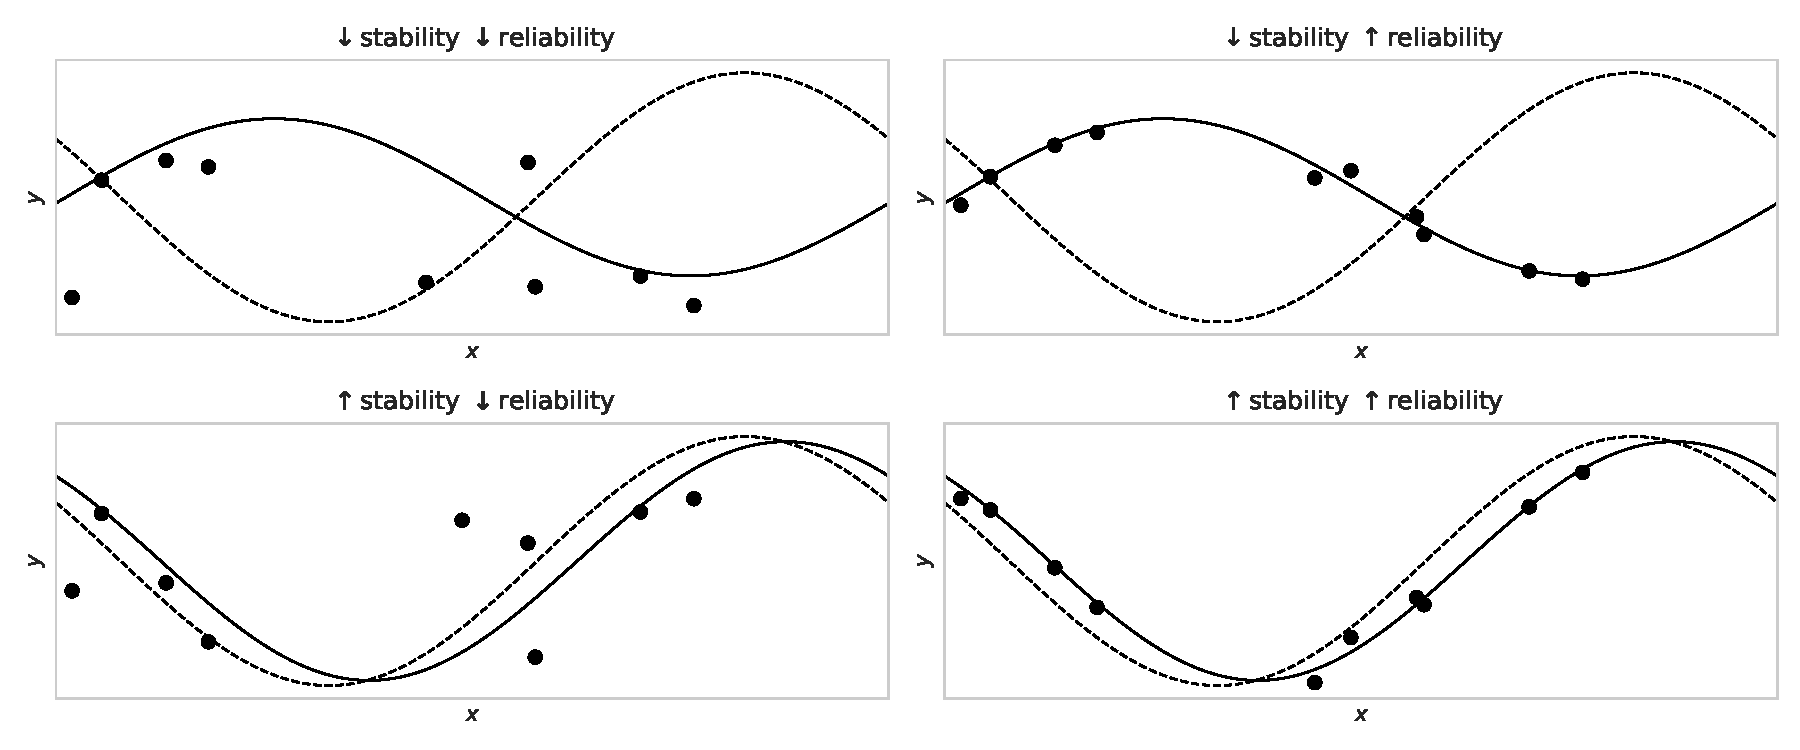
\includegraphics[width=0.99\linewidth]{figures/sinusoid_task.pdf}
  \caption{Sinusoid regression under varying predictability conditions. Each panel shows prompt examples (black dots) for a given target function at timestep $t$ (solid line), and the function at the preceding timestep $t-1$ (dashed line). Top row depicts volatile environments, meaning the target function changes significantly at each step. Bottom row depicts stable environments, where the target function is more stable across time. Left column depicts unreliable cues, where prompt examples are noisy. Right column depicts reliable cues, where prompt examples are less noisy and closer to the target function.}
  \label{fig:sinusoid_task}
\end{figure}

\textbf{Cue reliability.} We manipulate this by adjusting the variance, $\sigma^2$, of the Gaussian observation noise $\delta_i \sim \mathcal{N}(0, \sigma^2)$ added to the prompt targets $y_i$. A lower $\sigma^2$ corresponds to higher cue reliability, as the prompt examples more faithfully reflect the true underlying function $f_t$.

\textbf{Environmental stability.} We manipulate this by controlling the parameter $\alpha$ in an AR(1) process that governs the evolution of the task parameters $\theta_t = [A_t, \phi_t]^\top$ across training steps $t$. The parameter $\alpha \in [0, 1]$ dictates the correlation between successive tasks, where $\alpha \approx 1$ indicates high stability. The update rule is given by:

\begin{equation}
\theta_t = \alpha \theta_{t-1} + (1-\alpha)\tilde{\theta}_t
\label{eq:sinusoid_ar1}
\end{equation}

where $\tilde{\theta}_t$ represents random innovations drawn from the base task priors: amplitude $A \sim \mathcal{U}[0.5, 1.5]$ and phase $\phi \sim \mathcal{U}[0, 2\pi]$. This formulation ensures mean-reversion towards the prior distribution, allowing us to vary stability without drifting outside the solvable task distribution.

% In sinusoid regression \cite{finn2017model}, the task is to predict the output of a sinusoid function $f_t(x) = A_t \sin(x + \phi_t)$ (see Figure \ref{fig:sinusoid_task}). Each episode consists of prompt $N=10$ examples $\{(x_i, y_i)\}_{i=1}^N$ (inputs $x_i$ are sampled uniformly from $[-\pi, \pi]$, and corresponding outputs are $y_i = f_t(x_i) + \delta_i$, where $\delta_i$ represents Gaussian observation noise specific to each prompt example -- simulates cue reliability) and a query $x_q$ where the model must predict $y_q = f_t(x_q)$. The underlying function $f_t$ varies between episodes (timesteps $t$) -- simulates environmental volatility.

% The first task requires the model to perform regression on points sampled from a sinusoidal function (see Figure \ref{fig:sinusoid_task}), a setup inspired by prior meta-learning studies \cite{finn2017model}.

% Each training batch corresponds to a single environmental timestep $t$. Within a batch, all training sequences are generated from the same true underlying sinusoid $f_t(x) = A_t \sin(x + \phi_t)$. This setup mirrors a population adapting to a common, evolving environment.

% For each sequence, the model is provided with $N=10$ prompt examples $\{(x_i, y_i)\}_{i=1}^N$. Inputs $x_i$ are sampled uniformly from $[-\pi, \pi]$, and corresponding outputs are $y_i = f_t(x_i) + \delta_i$, where $\delta_i$ represents Gaussian observation noise specific to each prompt example. The model's objective is to predict the noise-free value $y_q = f_t(x_q)$ for a given query input $x_q$.

% \begin{figure}[!ht]
%   \centering
%   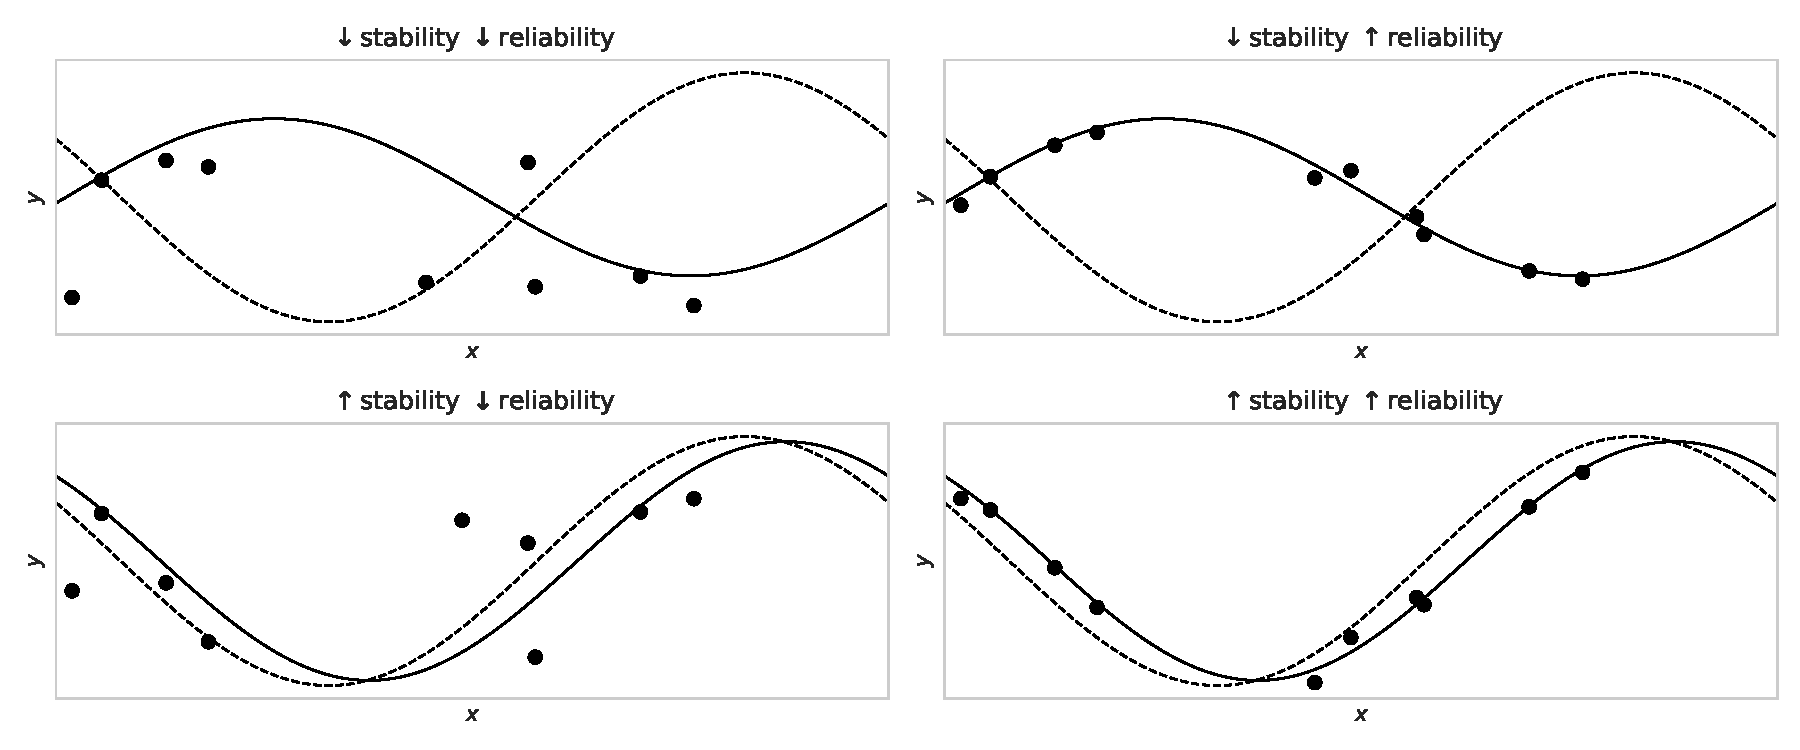
\includegraphics[width=0.99\linewidth]{figures/sinusoid_task.pdf}
%   \vspace{-0.5em}
%   \caption{Illustration of the sinusoid regression task under varying predictability conditions. Each panel shows prompt examples (black dots) for a given underlying sinusoid at timestep $t$ (solid line), and the sinusoid at the preceding timestep $t-1$ (dashed line). Top row: Low environmental stability, meaning the underlying sinusoid (solid line) changes significantly at each step. Bottom row: High environmental stability, where the underlying sinusoid is more stable across time. Left column: Low cue reliability, where prompt examples are noisy. Right column: High cue reliability, where prompt examples are less noisy and closer to the true underlying sinusoid.}
%   \label{fig:sinusoid_task}
% \end{figure}

% \textbf{Cue reliability.} This is manipulated by adjusting the variance, $\sigma^2_{\text{reliability}}$, of the Gaussian observation noise $\delta_i \sim \mathcal{N}(0, \sigma^2_{\text{reliability}})$ applied to the $y_i$ values in the prompt. Lower $\sigma^2_\text{reliability}$ corresponds to higher cue reliability.%, meaning prompt examples are more faithful to the true underlying sinusoid $f_t(x)$.

% \textbf{Environmental stability.} This is manipulated by controlling the parameter $\alpha_{\text{stability}}$ in an AR(1) process governing the evolution of the sinusoid parameters $\theta_t = [A_t, \phi_t]^T$ across successive environmental timesteps $t$. A higher $\alpha_{\text{stability}}$ indicates greater stability. The parameter update rule is:
% \begin{equation}
% \theta_t = \alpha_{\text{stability}} \theta_{t-1} + (1-\alpha_{\text{stability}})\theta_{\text{innovation}}^{(t)}
% \label{eq:sinusoid_ar1}
% \end{equation}
% where $\theta_0$ is initially sampled from prior distributions. For each subsequent timestep $t$, $\theta_{\text{innovation}}^{(t)}$ is a vector of innovations drawn afresh from these same priors:
% amplitude $A \sim U[0.5, 1.5]$ and phase $\phi \sim U[0, 2\pi]$. This formulation ensures mean-reversion towards the center of the prior distributions, with $\alpha_{\text{stability}}$ dictating the rate of change.

\subsection{Omniglot classification}

We adapt the few-shot Omniglot benchmark \cite{lake2015human} to construct a dynamic binary classification task (see Figure \ref{fig:omniglot_task}). At each training step $t$, a global mapping $M_t: \mathcal{C} \rightarrow \{0, 1\}$ assigns a hidden binary label to every character class $c$ in the Omniglot vocabulary $\mathcal{C}$ ($|\mathcal{C}| = 1623$). We define the target function $f_t(x) = M_t(c_x)$, where $c_x$ is the character class of image $x$.

Each episode consists of a prompt with $N=2$ image-label pairs $\{(x_i, y_i)\}_{i=1}^N$ and a query image $x_q$. The query image belongs to character class $c_q$, and the model must predict its current true label $M_t(c_q)$. Crucially, we construct the prompt such that one example matches the query's class ($c_k = c_q$). This setup explicitly creates a competition between strategies: the model can solve the task via ICL (copying the label $y_k$ from the matching prompt example) or via IWL (relying on the mapping $M_t(c_q)$ stored in its weights).

\begin{figure}[!ht]
  \centering
  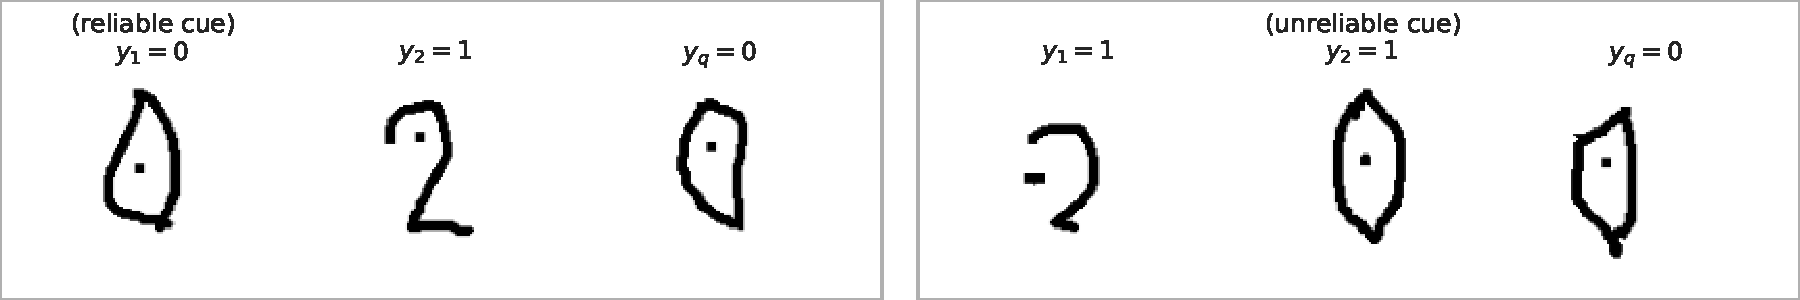
\includegraphics[width=0.99\linewidth]{figures/omniglot_task.pdf}
  \caption{Omniglot classification episodes. The prompt on the left contains a reliable cue (prompt label $y_1$ for character $c_1=c_q$ matches $M_t(c_q)$). The prompt on the right contains an unreliable cue (prompt label $y_2$ for $c_2=c_q$ is flipped relative to $M_t(c_q)$).}
  \label{fig:omniglot_task}
\end{figure}

\textbf{Cue reliability.} We operationalize reliability by controlling the probability, $\rho$, that prompt labels are accurate. For each example $i$ in the prompt, the provided label $y_i$ corresponds to the true mapping $M_t(c_i)$ with probability $\rho$, and is flipped otherwise:
\begin{equation}
y_i = \begin{cases} 
M_t(c_i) & \text{with probability } \rho \\
1 - M_t(c_i) & \text{with probability } 1 - \rho
\end{cases}
\label{eq:omniglot_reliability}
\end{equation}

\textbf{Environmental stability.} We operationalize stability by controlling the persistence of the global mapping $M_t$ over time. The initial mapping $M_0(c)$ is sampled from a Bernoulli(0.5) distribution. For subsequent steps $t > 0$, each character's label persists with probability $\gamma$:
\begin{equation}
M_t(c) = \begin{cases} 
M_{t-1}(c) & \text{with probability } \gamma \\
1 - M_{t-1}(c) & \text{with probability } 1 - \gamma
\end{cases}
\label{eq:omniglot_stability}
\end{equation}
A higher $\gamma$ indicates greater stability. This process induces a first-order temporal autocorrelation of $\alpha = 2\gamma - 1$ for each character's label trajectory.

% The second task is few-shot binary classification of Omniglot characters \cite{lake2015human} (see Figure \ref{fig:omniglot_task}). Similar to the sinusoid task, each training batch corresponds to a single environmental timestep t. At each timestep $t$, an underlying global mapping, $M_t: \mathcal{C} \rightarrow \{0, 1\}$, assigns a binary label to each character $c$ from a set $\mathcal{C}$ of 1623 unique Omniglot character classes.

% A prompt sequence comprises $N=2$ example image-label pairs $\{(x_i, y_i)\}_{i=1}^N$, followed by a query image $x_q$ (an exemplar of character class $c_q$). The model predicts the true binary label $M_t(c_q)$. Critically, one example character in the prompt, $c_k$, matches the query's class $c_k=c_q$. This allows the model to predict the query label by relying on the in-context label $y_k$ (ICL) or by accessing an internalized representation of $M_t(c_q)$ (IWL).

% \begin{figure}[!ht]
%   \centering
%   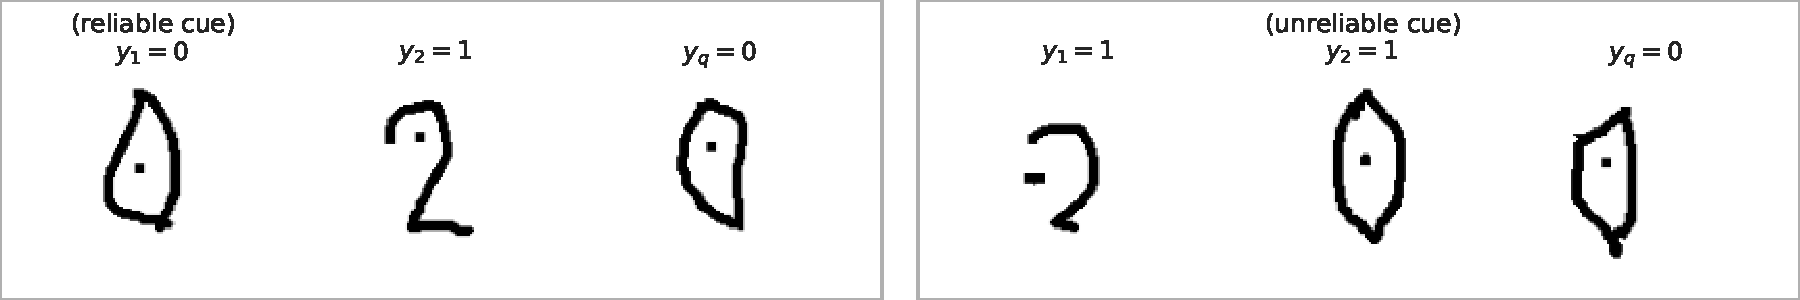
\includegraphics[width=0.99\linewidth]{figures/omniglot_task.pdf}
%   \vspace{-0.5em}
%   \caption{Sequences drawn from the Omniglot binary classification task. (\textbf{Left}) A sequence illustrating a reliable in-context cue (prompt label $y_1$ for character $c_1=c_q$ matches $M_t(c_q)$). (\textbf{Right}) A sequence illustrating an unreliable in-context cue (prompt label $y_2$ for $c_2=c_q$ is flipped relative to $M_t(c_q)$).}
%   \label{fig:omniglot_task}
% \end{figure}

% \textbf{Cue reliability.}
% This is manipulated by controlling the probability, $p_\text{reliability}$, that the label $y_i$ for a prompt character $c_i$ matches its true label $M_t(c_i)$. Specifically:
% \begin{equation}
% y_i = \begin{cases} 
% M_t(c_i) & \text{with probability } p_{\text{reliability}} \\
% 1 - M_t(c_i) & \text{with probability } 1 - p_{\text{reliability}}
% \end{cases}
% \label{eq:omniglot_reliability}
% \end{equation}
% Higher $p_\text{reliability}$ indicates higher cue reliability.

% \textbf{Environmental stability.}
% This is manipulated by varying the probability, $p$, that the true mapping $M_t(c)$ for each character $c$ persists from the previous timestep $M_{t-1}(c)$. The initial mapping $M_0(c)$ is sampled from Bernoulli(0.5) for all characters. For $t>0$:
% \begin{equation}
% M_t(c) = \begin{cases} 
% M_{t-1}(c) & \text{with probability } p \\
% 1 - M_{t-1}(c) & \text{with probability } 1 - p
% \end{cases}
% \label{eq:omniglot_stability}
% \end{equation}
% Higher $p_\text{stability}$ signifies greater environmental stability. The first-order temporal autocorrelation for each character's label in this process is 
% $\alpha=2p-1$.
% ranging from -1 (perfect anti-correlation if $p_\text{stability}=0$) to 1 (perfect stability if $p_\text{stability}=1$).

\subsection{Model and training}

% Drawing on the previous literature, we use both a sinusoid regression task \cite{finn2017model} and an Omniglot classification task \cite{lake2015human}.
All experiments use a decoder-only Transformer with 4 layers, 4 attention heads per layer, an embedding dimension of 128, and learned positional encodings.
Input processing varies by task. For the sinusoid regression task, scalar inputs and outputs are linearly projected to the embedding dimension. For Omniglot classification, character images are processed by a shallow ResNet with three stages, each with 2 residual blocks, and outputting 16, 32, and 64 channels per stage, respectively. This ResNet is trained jointly with the Transformer.

Models are optimized to minimize either the mean squared error (MSE) for sinusoid regression or the binary cross-entropy (BCE) for Omniglot classification, calculated on their predictions for the query item ($y_q$). We use the AdamW optimizer \cite{loshchilov2017decoupled} with a peak learning rate of $1 \times 10^{-4}$, subject to a cosine decay schedule following 1,000 warmup steps. All models are trained for a total of 50,000 training steps, using a batch size of 128.

\subsection{Evaluation}

To quantify the model's preference for ICL versus IWL, we use an evaluation protocol inspired by \citet{chan2022data}. This involves constructing evaluation prompts where the underlying target task explicitly conflicts with the current training environment.

\textbf{Evaluation prompts.} We generate these prompts by sampling an evaluation task, $f_e$, from the prior distribution such that it is independent of the current training task, $f_t$. We then construct a prompt $\{(x_i, y_i)\}_{i=1}^N$ using labels derived from this evaluation task ($y_i = f_e(x_i)$).

\textbf{Target definitions.} For a given query $x_q$, this setup defines two conflicting prediction targets:
\begin{itemize}
    \item The ICL target, $y_\text{ICL}=f_e(x_q)$, corresponds to the label implied by the prompt; a model predicting this value is relying on context (ICL).
    \item The IWL target, $y_\text{IWL}=f_t(x_q)$, corresponds to the label implied by the current training environment; a model predicting this value disregards the prompt in favor of its weight-based encoding of the environment (IWL).
\end{itemize}

\textbf{Quantifying strategy preference.} We quantify the model's strategy preference by computing the prediction error relative to both targets ($E_\text{ICL}$ and $E_\text{IWL}$) using the task-appropriate metric (MSE for Sinusoid, BCE for Omniglot). We define the ICL preference score as:
\begin{equation}S_\text{ICL} = \frac{E_\text{IWL}}{E_\text{ICL} + E_\text{IWL}}\label{eq:s_icl_preference}\end{equation}
An $S_\text{ICL} \approx 1$ indicates pure reliance on context, while $S_\text{ICL} \approx 0$ indicates pure reliance on weights.
% This metric captures strategy preference, not absolute task performance.

% To assess a trained model's preference for ICL versus IWL solutions, we employ a targeted evaluation protocol inspired by prior work \cite{chan2022data}. This evaluation is performed periodically during training. It uses novel evaluator tasks sampled from the same prior distributions as the training tasks but unseen during training. This allows us to contrast mappings learned in weights against those learnable from context during evaluation.

% \textbf{Evaluator tasks.} 
% For sinusoid regression, an evaluator task is a specific function $f_e(x) = A_e \sin(x + \phi_e)$ with $(A_e, \phi_e)$ newly sampled from their priors (Section \ref{sec:experimental_design_sinusoid}).
% For Omniglot classification, an evaluator task is a complete binary mapping $M_e: \mathcal{C} \rightarrow \{0, 1\}$ where each $M_e(c)$ is independently sampled from Bernoulli(0.5).
% For each evaluator task ($f_e$ or $M_e$) and a query input $x_q$, we construct a noiseless evaluation prompt $P_e = \{(x_j, y_j)\}_{j=1}^{N}$, with examples derived directly from $f_e$ or $M_e$. For Omniglot, one example in $P_e$ matches $c_q$. The model then predicts $\hat{y}_q$ (sinusoid) or $\hat{p}_q = P(y_q=1 | P_e, x_q)$ (Omniglot).

% \textbf{Evaluator targets.}
% At the moment of periodic evaluation, we define two conflicting targets for the model's prediction:
% \begin{itemize}
%     \item \textbf{ICL target:} The ground-truth for $x_q$ from the current evaluator task: $f_e(x_q)$ or $M_e(c_q)$. This target is independent of the training environment's state.
%     \item \textbf{IWL target}: The ground-truth for $x_q$ from the current state of the training environment generator (i.e., $f_t(x_q)$ or $M_t(c_q)$ at the time of evaluation). This reflects what a model relying purely on an internalized representation of the latest training environment state would predict.
% \end{itemize}

% \textbf{Quantifying preference.}
% We calculate the model's prediction error relative to both targets ($E_\text{ICL}$ and $E_\text{IWL}$) using mean squared error (sinusoid) or binary cross-entropy (Omniglot). A model prefers ICL if $E_\text{ICL} > E_\text{IWL}$. We quantify this preference using the score:
% \begin{equation}
%     S_\text{ICL} = \frac{E_\text{IWL}}{E_\text{ICL} + E_\text{IWL} + \epsilon}
% \label{eq:s_icl_preference}
% \end{equation}
% where $\epsilon$ (e.g., $1 \times 10^{-8}$) ensures numerical stability. $S_\text{ICL} > 0.5$ indicates ICL preference. This metric captures strategy preference, not absolute task performance.

% Further details and standard performance metrics are in the appendix.

\section{Results}
\label{sec:analysis}

Our experiments reveal that the learning strategies adopted by Transformers are systematically shaped by the predictability of their training environment, in ways that closely parallel adaptive mechanisms in evolutionary biology.
We first examine how environmental stability and cue reliability governs the asymptotic preference for ICL versus IWL. We then explore the learning dynamics between these strategies, revealing task-dependent patterns of transience (ICL $\to$ IWL and vice versa). Finally, we show that the cost of acquiring ICL versus IWL governs these dynamics. Together, these results reconcile a diverse set of learning phenomena in Transformers with
principles of biological adaptation.

\begin{figure}[!ht]
  \centering
  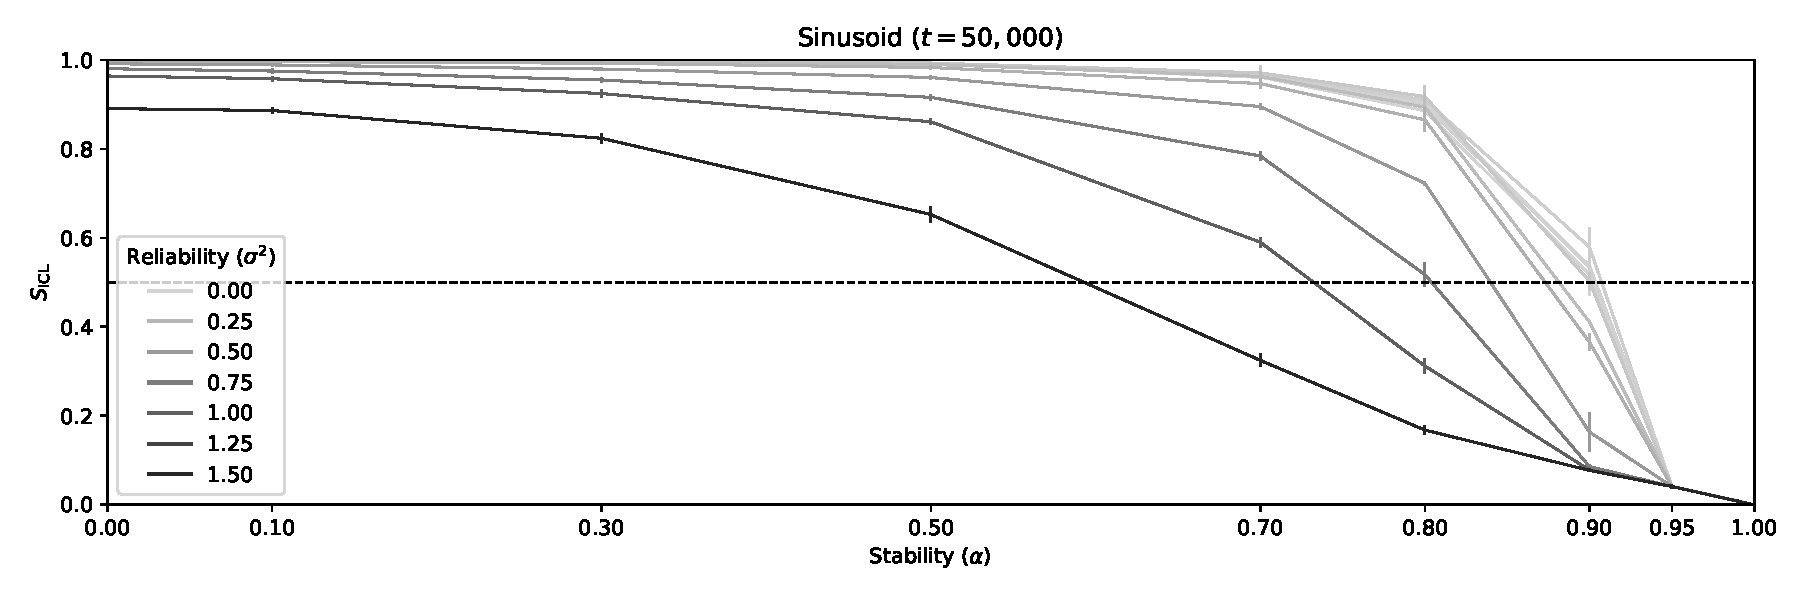
\includegraphics[width=0.99\linewidth]{figures/sinusoid_asymptotic.pdf}
  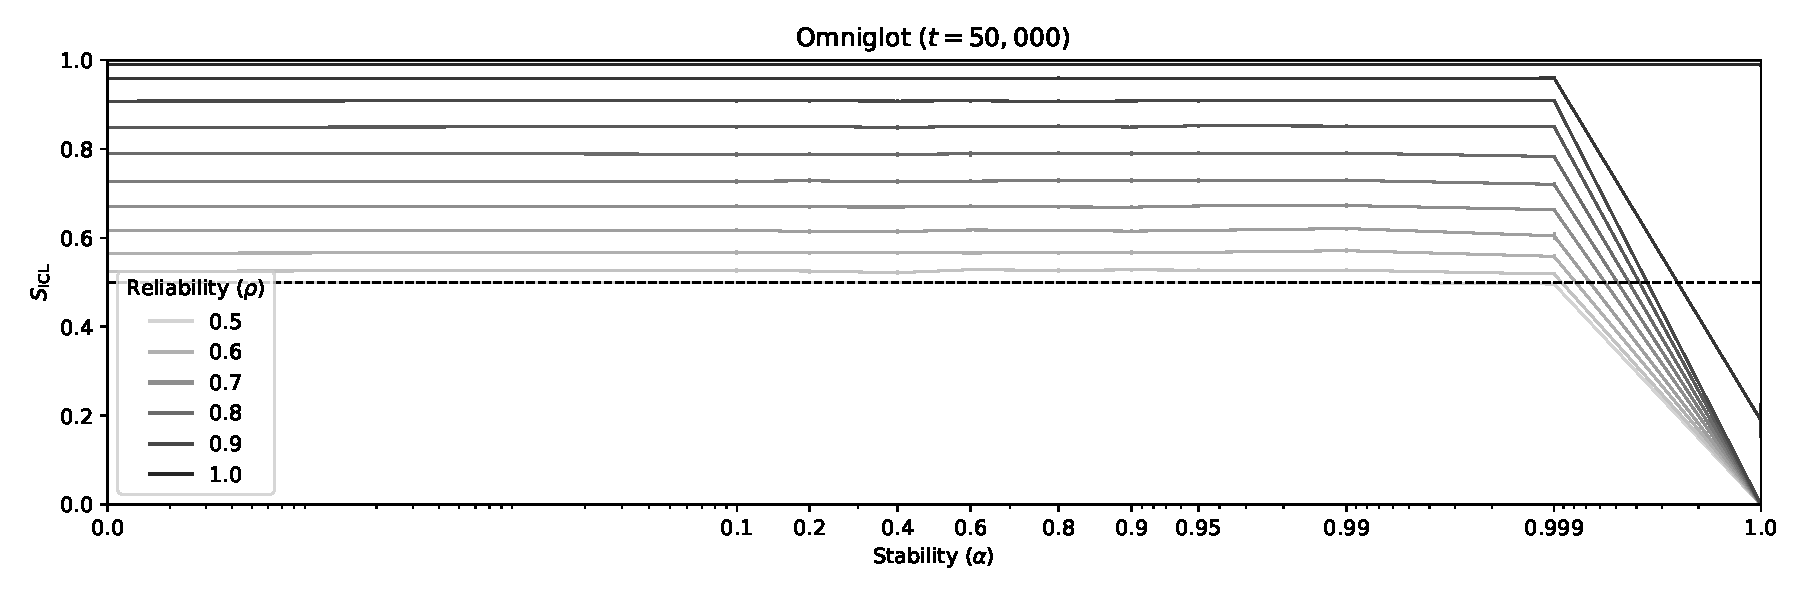
\includegraphics[width=0.99\linewidth]{figures/omniglot_asymptotic.pdf}
  \caption{
    The asymptotic strategy of converged models ($t = 50,000$).
    The ICL preference score ($S_\text{ICL}$) is plotted as a function of environmental stability (x-axis) and cue reliability (line brightness).
    The dashed line at $S_\text{ICL} = 0.5$ marks the crossover point.
    In sinusoid regression (top), stability is parameterized by the AR(1) coefficient $\alpha$. Cue reliability increases with decreasing noise variance $\sigma^2$ (lighter lines).
    In Omniglot classification (bottom), stability is parameterized by the mapping persistence $\alpha$ (logit scale). Cue reliability increases with label correctness probability $\rho$ (lighter lines).
  }
  \label{fig:asymptotic}
\end{figure}

\subsection{Determinants of asymptotic strategy}
\label{sec:asymptotic}

Figure~\ref{fig:asymptotic} shows how dimensions of environmental predictability influence the model's asymptotic strategy ($t = 50,000$), supporting our core hypothesis that information reliability across timescales governs the trade-off between ICL and IWL.

\textbf{Stable environments favor ICL.}
In sinusoid regression (Figure~\ref{fig:asymptotic}, top), increasing environmental stability ($\uparrow\alpha$) leads to a precipitous decline in ICL preference. As $\alpha \to 1$, the model shifts almost entirely to IWL. This recapitulates the biological principle of genetic assimilation: when environmental features are stable across generations, selection favors the permanent encoding of traits over incurring cost of plasticity \cite{stearns1989evolutionary,dewitt1998costs}. Similarly, in the Omniglot task (Figure~\ref{fig:asymptotic}, bottom), ICL preference plummets as $\alpha \to 1$. This reflects a transition where the global mapping becomes invariant, allowing the model to consolidate the task into its weights and render the prompt redundant.

\textbf{Volatile environments with reliable cues favor ICL.}
Conversely, when environmental stability is low, the model relies heavily on ICL, provided that reliable cues are available. In sinusoid regression, reliable cues ($\downarrow\sigma^2$, lighter lines) fosters strong ICL preference. This aligns with the evolutionary view that plasticity is favored specifically when environmental fluctuations render fixed traits maladaptive, but only if accurate cues exist to guide the plastic response \cite{stephens1989variance,scheiner1993genetics}.
In Omniglot, this effect is even more pronounced: across a broad range of instability ($\alpha < 0.95$), cue reliability is the primary determinant of strategy.

\textbf{When strategies are equally effective.}
Interestingly, we observe a deviation from biology in the Omniglot task. With perfectly reliable cues ($\rho = 1$), the model maintains a strong preference for ICL even when the environment is perfectly stable (Figure~\ref{fig:asymptotic}, bottom right). Evolutionary theory suggests that plasticity is selected against in stable environments due to maintenance costs \cite{dewitt1998costs}. The persistence of ICL here implies that, for Transformers, the maintenance cost of ICL may be negligible --- or, crucially, that the acquisition cost of the alternative strategy (IWL) is prohibitively high. This suggests that when both strategies are asymptotically effective, the model's preference is driven by the difficulty of learning each solution. We formalize this intuition in Section~\ref{subsec:relative_cost_hypothesis}.

\begin{figure}[!ht]
  \centering
  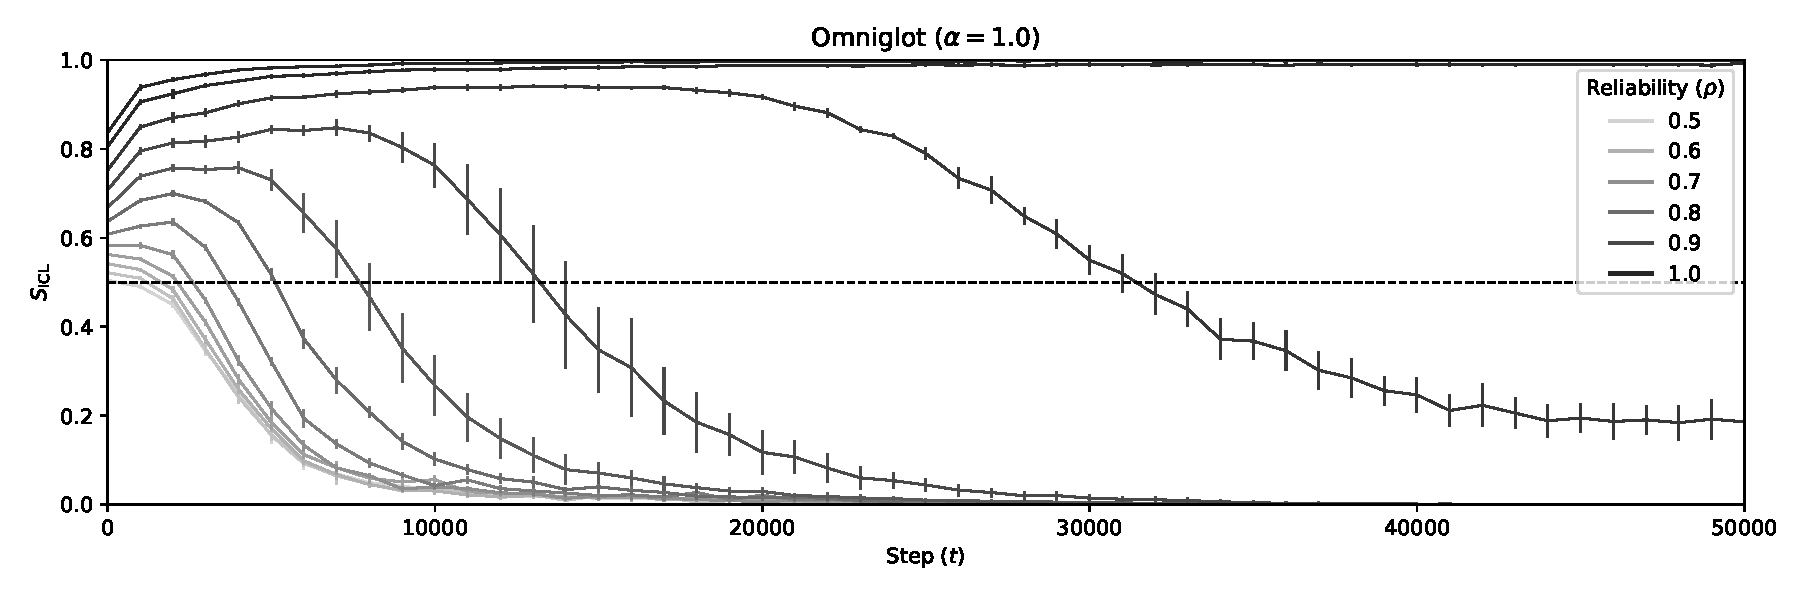
\includegraphics[width=0.99\linewidth]{figures/omniglot_transience.pdf}
  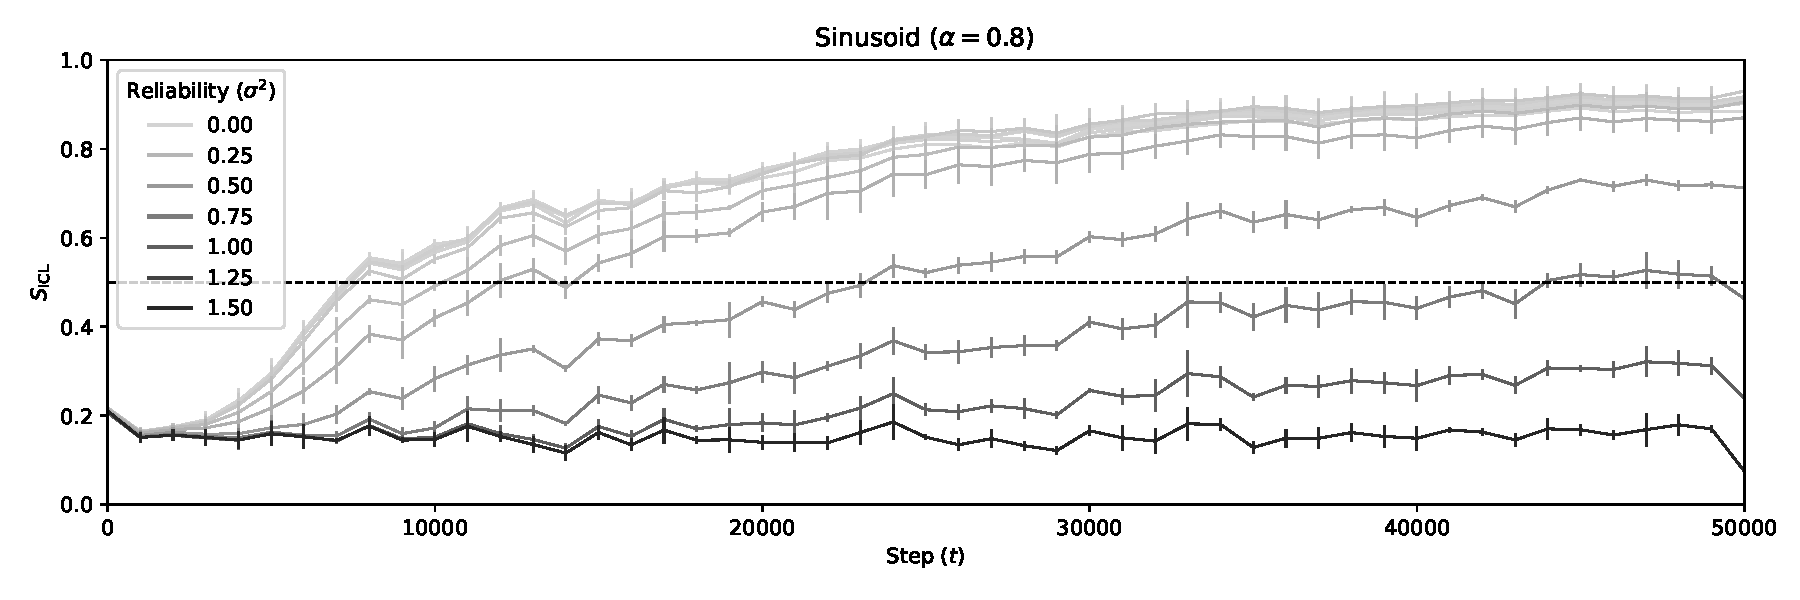
\includegraphics[width=0.99\linewidth]{figures/sinusoid_transience.pdf}
  \vspace{-0.5em}
  \caption{
  % Learning dynamics and transience.
  The shift in ICL preference ($S_\text{ICL}$) over training steps ($t$) reveals opposing directions of transience. Omniglot classification (top) demonstrates ICL transience ($\alpha=1$). The model initially relies on ICL but gradually consolidates the task into weights. Sinusoid regression (bottom) demonstrates IWL transience ($\alpha=0.8$). The model initially relies on IWL but gradually improves inferences by using the prompt.
  }
  \label{fig:transience}
\end{figure}

\subsection{Task-dependent patterns of transience}
\label{sec:transience}

Beyond asymptotic strategies, the learning trajectories reveal shifts in strategy preference during training --- a phenomenon known as \textit{transience} \cite{singh2023transient,panwar2023context,singh_strategy_2025}. As shown in Figure~\ref{fig:transience}, the direction of change between ICL and IWL is highly task-dependent.

\textbf{ICL transience (ICL $\to$ IWL).} In the Omniglot task under high environmental stability (Figure~\ref{fig:transience}, top), we observe the phenomenon of ICL transience \cite{singh2023transient}. The model exhibits a strong preference for ICL early in training. However, as training progresses, the model gradually shifts towards an IWL solution. This progression parallels genetic assimilation, where a trait initially induced by environmental cues (plasticity) becomes genetically encoded under prolonged, stable selection, eventually rendering the cue redundant \cite{waddington1953genetic, pigliucci2006phenotypic}.

\textbf{IWL transience (IWL $\to$ ICL).} In contrast, the sinusoid regression task (Figure~\ref{fig:transience}, bottom) exhibits the opposite trajectory: IWL transience (or delayed ICL). Under medium stability ($\alpha=0.8$), the model initially relies on IWL (approximating the function via weights) and exhibits a low preference for context. A strong preference for ICL emerges only later in training, particularly when cues are highly reliable ($\downarrow\sigma^2$). This suggests that for sinusoid regression, an IWL approximation of the target function is easier to learn early on, whereas the circuitry required for ICL develops more slowly. This pattern relates to phenomena like \textit{grokking}, where generalization capability (here, ICL) emerges abruptly after a long period of fitting the training distribution \cite{power2022grokking}.

\subsection{Cost-based arbitration between strategies}
\label{subsec:relative_cost_hypothesis}

The contrasting trajectories observed in Section~\ref{sec:transience} raise the question of why Transformers initially prefer ICL in Omniglot (ICL $\to$ IWL), but IWL in Sinusoid (IWL $\to$ ICL). These results suggest that learning dynamics are governed not only by the asymptotic optimality of a strategy (which is determined by the environment), but also by the cost of acquiring that strategy. We posit that the strategy that is cheaper to learn (i.e., whose inductive bias closely fits the task structure) will emerge earlier in training, regardless of whether it is the long-term optimal solution.
This aligns with the broader literature on \textit{simplicity bias}~\cite{arpit2017closer,goldblum2023no,deora2025context}, while highlighting that simplicity is contingent on the correspondence between the model and the training data.

\textbf{Cost of learning for each strategy.}
Intuitively, the relative difficulty of IWL and ICL differs across our two tasks.
In Omniglot, IWL requires memorizing a global mapping for a large vocabulary ($|\mathcal{C}| = 1623$). This is a high-capacity memorization problem with high sample complexity. In contrast, ICL requires only a local pattern-matching circuit (comparing the query to the prompt) \cite{olsson2022context, singh_what_2024}, which is simple for the attention mechanism to discover. Thus, for Omniglot, ICL is cheaper than IWL.
In sinusoid regression, the dynamic is reversed. An IWL solution requires learning a single global sine wave approximation, which neural networks can parameterize rapidly. Conversely, ICL requires implementing a regression algorithm within the forward pass (e.g., gradient descent or ridge regression via attention \cite{von2023transformers}). This is a complex circuit that is difficult to learn. Thus, for sinusoid, IWL is cheaper than ICL.

\textbf{Quantifying learning cost.} To formalize this intuition, we adopt the minimum description length (MDL) perspective for quantifying the cost of learning a particular dataset, using the \textit{prequential codelength} \cite{blier2018description}.
Prequential codelength is the cumulative negative log-likelihood (NLL) of each token, computed sequentially by a model strategy (ICL or IWL) trained on all preceding tokens. See Appendix~\ref{sec:prequential} for a formal description. Intuitively, a strategy that is easier to learn for the particular dataset (more aligned inductive bias) will achieve lower log-likelihoods early in training, resulting in a shorter prequential codelength.\footnote{Prequential codelength also exhibits a ``catch-up phenomenon'' that may be interesting to compare with our transience observations here --- complex models have higher cost initially and later require more samples to ``catch up'', even after they become more optimal \cite{erven_catching_2012}.}

Because our goal is to evaluate the inductive bias of different learning strategies the transformer can adopt (ICL or IWL), rather than the Transformer as a whole, we consider training environments where either ICL or IWL are strongly favored. For ICL, this means a volatile environment ($\alpha=0.0$) with reliable cues ($\rho=1.0, \sigma^2=0.0$). And for IWL, this means a stable environment ($\alpha=1.0$) with unreliable cues ($\rho=0.5, \sigma^2=1.5$). We then computed the prequential codelength of each strategy (ICL and IWL) for each task (sinusoid and Omniglot) by keeping a running sum of the NLL (i.e., the loss) during the entire course of training.\footnote{It is worth noting that for the Omniglot task, the binary cross-entropy loss is equivalent to the NLL; however for sinusoid regression, the mean squared error loss is monotonically related to the NLL under a Gaussian likelihood.}
As shown in Figure~\ref{fig:coding_cost}, the results confirm our intuition. For Omniglot, the cost for ICL is significantly lower than for IWL. Conversely, for sinusoid, the cost for IWL is significantly lower than for ICL. This metric predicts the starting point of the learning trajectories in Figure~\ref{fig:transience} --- the model adopts the cheaper strategy first.

\begin{figure}[!ht]
  \centering
  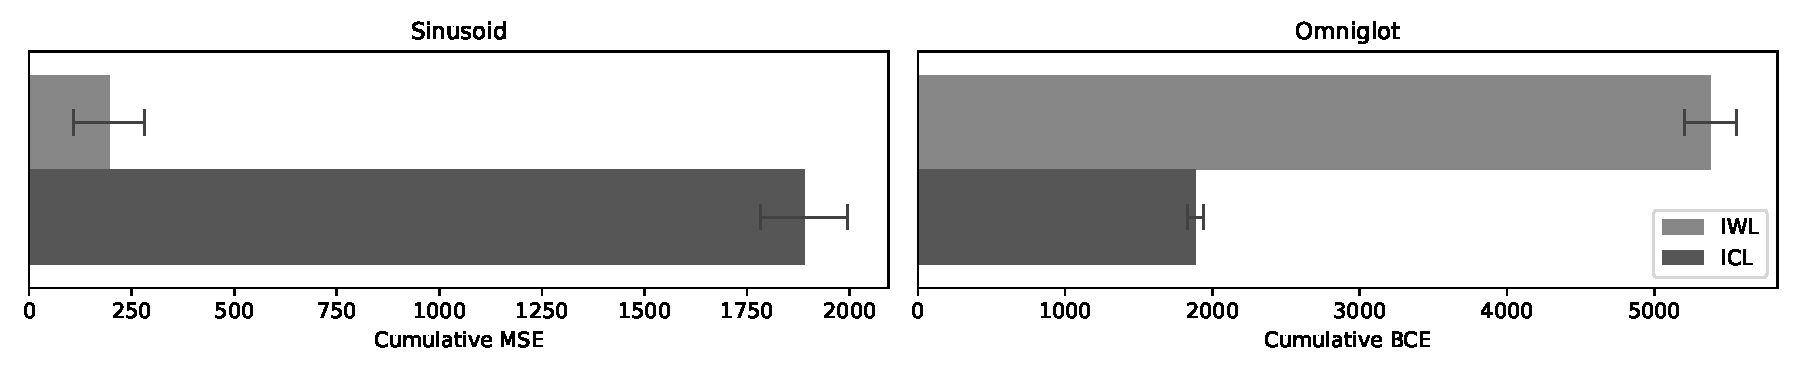
\includegraphics[width=0.99\linewidth]{figures/coding_cost.pdf}
  \caption{Cost of learning IWL vs ICL, measured as the prequential codelength (cumulative MSE/BCE loss accrued over 50,000 training steps). IWL is less expensive than ICL for Sinusoid, and the reverse is true for Omniglot, showing that the relative cost of IWL vs ICL corresponds to transience dynamics (IWL-first or ICL-first) observed experimentally for the two tasks.}
  \label{fig:coding_cost}
\end{figure}


\textbf{Manipulating learning cost.}
To causally validate that learning cost drives these dynamics, we manipulated the difficulty of the IWL strategy in the Omniglot task. The sample complexity of IWL (memorizing labels for all characters) is governed by the coupon collector problem --- to see all $N=|\mathcal{C}|$ characters at least $K$ times requires $\Theta(KN \log N)$ episodes. By reducing the vocabulary size $|\mathcal{C}|$, we reduce the cost of the IWL strategy.

As Figure~\ref{fig:reversal} shows, reducing $|\mathcal{C}|$ from 1623 to 100 drastically changes the learning dynamics. In the standard setting (dark line), the model starts with high ICL preference. However, in the reduced setting (lightest line), the dynamics reverse: the model starts with a preference for IWL ($S_\text{ICL} < 0.2$) before eventually switching to ICL. This induced IWL transience (reproducing the dynamic seen in the Sinusoid task) shows that the initial preference of a strategy is determined by its acquisition cost.

\begin{figure}[!ht]
  \centering
  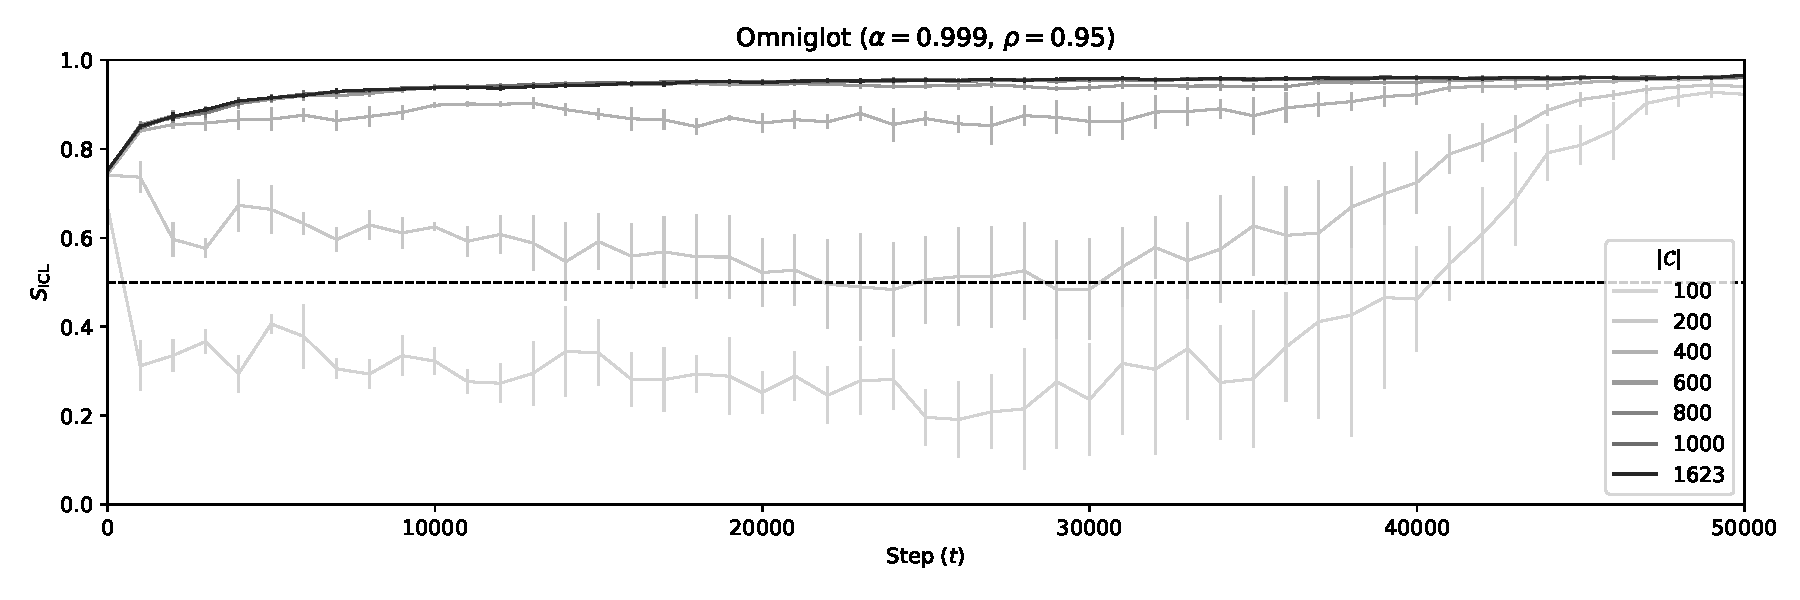
\includegraphics[width=0.99\linewidth]{figures/omniglot_reversal.pdf}
  \caption{
    % \textbf{Causal validation of acquisition cost.}
    We manipulate the learning cost of the IWL strategy by varying the Omniglot vocabulary size ($|\mathcal{C}|$).
    We plot ICL preference ($S_\text{ICL}$) across training steps ($t$) in a stable environment ($\alpha=0.999$) with reliable cues ($\rho=0.95$).
    In the standard setting ($|\mathcal{C}|=1623$, dark line), the model exhibits a sustained preference for ICL.
    Drastically reducing the vocabulary size (e.g., to $|\mathcal{C}|=100$, lightest line) lowers the cost of IWL, causing the model initially favors IWL before eventually switching to ICL, thereby reversing the pattern of transience previously observed in this task.
  }
  \label{fig:reversal}
\end{figure}


Our findings align with recent work linking ICL transience to task structure \cite{singh2023transient} and relative acquisition speeds \cite{nguyen_differential_2024,singh_strategy_2025,wurgaft2025context}, as well as mechanistic studies on circuit efficiency  and competition dynamics \cite{thilak_slingshot_2022, nanda_progress_2023, varma_explaining_2023,park2024competition}. Together, they imply that Transformers arbitrate between strategies based on a distinct optimization cost. The framework of {\em resource rational analysis} \cite{lieder2020resource}, introduced in cognitive science but inspired by earlier work in AI \cite{horvitz1987reasoning,russell1994provably}, may provide a set of tools for formalizing this tradeoff and offering further insight into the behavior of AI models. 

\section{Discussion}

In this paper, we have demonstrated that the competition between ICL and IWL in Transformers is governed by the same principles of environmental predictability that shape biological adaptation. While stability and cue reliability dictate the asymptotic strategy (favoring IWL or ICL, respectively), our analysis of transience reveals that the trajectory of learning is driven by the cost of acquiring each strategy. We find that Transformers consistently adopt the easier strategy first (as determined by their inductive bias for a particular task) while the more costly but asymptotically optimal strategy develops over a longer timescale.

% Our investigation, drawing analogies from evolutionary biology, has demonstrated that core principles of environmental predictability systematically govern the balance and dynamics between in-context learning (ICL) and in-weights learning (IWL) in Transformer models. We found that high environmental stability strongly promotes IWL, mirroring the selection for genetically fixed traits in stable biological environments, while high cue reliability enhances ICL efficacy, akin to phenotypic plasticity's reliance on dependable environmental signals. Furthermore, our findings revealed distinct, task-dependent transience patterns: models sometimes shift from ICL to IWL (resembling genetic assimilation) or, conversely, from IWL to ICL (resembling the evolution of plasticity). We proposed and provided evidence for a relative-cost hypothesis, suggesting these dynamics are driven by the comparative ease of learning and implementing each strategy within a given model and task context. These results affirm the utility of an evolutionary lens for understanding adaptive learning in artificial neural networks.

\subsection{Limitations and future directions}
\label{sec:limitations}

While this work offers foundational insights into the learning dynamics of Transformers, we acknowledge specific limitations that define its scope, as well as promising avenues for future research.

\textbf{Task simplification.} Our sinusoid and Omniglot environments are, by design, simplifications of the complex linguistic environments that LLMs are trained in. However, such controlled settings are essential for isolating variables (e.g., environmental predictability) and their causal influence on learning dynamics. Future work should aim to verify these principles in more complex domains.
% The sinusoid regression and Omniglot classification tasks are, by design, simplifications of the complex, high-dimensional environments (e.g., natural language) where large language models typically operate. Such controlled settings are, however, essential for isolating variables and establishing clearer causal links between predictability and learning dynamics. They provide a foundational understanding that can inform future investigations in more complex domains.


\textbf{Levels of analysis.}
Our framework constitutes a computational-level analysis \cite{marr82vision, ku2025using}. We characterize the adaptive problem a system faces (optimizing prediction under varying uncertainty) and the functional logic of its solution (ICL vs. IWL). The analogy to evolutionary biology operates at this functional level of adaptation to statistical structure in the environment; we do not claim a direct mechanistic equivalence between IWL and ICL in Transformers and the specific genetic or developmental pathways of biological adaptation.


\textbf{The Baldwin effect.}
Beyond merely managing uncertainty, a key evolutionary function of plasticity is to accelerate adaptation on rugged fitness landscapes (the \textit{Baldwin Effect}). Plasticity smooths the fitness landscape by enabling individuals to survive in new environments, guiding the population toward regions where genetic assimilation can subsequently fix the trait \cite{hinton1987learning, fernando2018meta}. An exciting direction for future research is to determine if an analogous dynamic exists in Transformers --- does the early emergence of ICL serve as a scaffold for accelerating the acquisition of IWL solutions for complex tasks?
% A key argument for biological plasticity, beyond managing uncertainty, is its potential to accelerate evolution on complex fitness landscapes (e.g., via the Baldwin Effect). Plastic individuals can more effectively explore and identify advantageous phenotypic regions, which can then be refined and genetically assimilated \cite{hinton1987learning,fernando2018meta}. An analogous question for Transformers is whether ICL not only provides flexibility but also speeds up the acquisition of robust IWL solutions for complex tasks, perhaps by IWL reusing or refining circuits initially developed for ICL \cite{singh_strategy_2025}.

\subsection{Conclusion}

By viewing Transformers through the lens of evolutionary biology, we show that their learning dynamics are governed by the statistical structure of their environments. We find that the preference for ICL versus IWL is strongly determined by dimensions of environmental predictability (specifically, environmental stability and cue reliability). Furthermore, our analysis of learning dynamics reveals that while the environment dictates the asymptotically optimal strategy, the learner's inductive bias leads to transient phases where the model exploits a lower-cost solution first. This framework establishes a more ecological perspective on model behavior, paving the way for training methodologies that cultivate systems capable of robustly and flexibly navigating the diverse and dynamic environments they increasingly encounter.

% This research underscores the significant value of applying an evolutionary lens to artificial intelligence, demonstrating that disparate adaptive systems—from biological organisms to Transformers—arrive at convergent solutions when facing analogous challenges. By characterizing how environmental predictability shapes the competition between ICL and IWL, we establish a more fundamental understanding of how models adapt to their training data. These insights pave the way for a new ecological perspective on model behavior, offering principled guidance for designing training methodologies that yield systems capable of robustly and flexibly navigating the diverse environments they increasingly encounter.

% This research underscores the significant value of drawing on established principles from evolutionary theory to illuminate complex learning behaviors in artificial systems. The insights gained not only contribute to a more fundamental understanding of how Transformers adapt to their training environments but also pave the way for designing more effective training methodologies -- bringing forth a more ecological perspective on model behavior. Ultimately, this line of inquiry can help guide the development of artificial systems capable of robustly and flexibly navigating the diverse and dynamic environments they increasingly encounter.

% \subsection{Future Directions}

% The current framework opens several exciting avenues for future research:

%\textbf{Types of Predictability and Uncertainty:}
%Uncertainty can stem from two primary sources: aleatory uncertainty (inherent environmental randomness) and epistemic uncertainty (arising from a lack of knowledge, reducible with more data or better models) \cite{der2009aleatory, kendall2017uncertainties,fox2011distinguishing}. Our manipulations of cue reliability (via noise) and environmental stability (via stochastic AR(1) processes) primarily addressed aleatory uncertainty. The influence of epistemic uncertainty -- for instance, how factors like the number of prompt examples ($N$) affect learning strategy -- remains an important area for future work. We held $N$, model size, and batch size constant to isolate the effects of our chosen predictability dimensions.


% Future experiments could, for instance, test if pre-training regimes that explicitly foster diverse ICL capabilities lead to more sample-efficient IWL on challenging downstream tasks.

% \textbf{Operationalizing predictability.}
% Our use of noise for cue reliability and AR(1) processes for environmental stability represents specific implementations of predictability. Future work should explore other forms of environmental structure and change. This includes systematically varying the nature of aleatory uncertainty beyond our current manipulations -- for example, by introducing non-stationary predictability or more complex temporal structures (e.g., environments with punctuated equilibria \cite{gould1977punctuated}).
% Furthermore, building on our distinction between uncertainty types, a crucial next step is to investigate the impact of epistemic uncertainty.
% This could involve manipulating the number of prompt examples ($N$), the diversity of tasks seen during pre-training, or other factors that affect the model's effective knowledge about the current task context.

% \textbf{Testing the Relative-Cost Hypothesis:}
% Our relative-cost hypothesis posits that the computational ease of learning, representing, and executing a strategy dictates choice and transience. A key avenue for deepening our understanding and rigorously testing this hypothesis lies in developing theoretical models to formalize these "computational costs." Such models could draw inspiration from algorithmic information theory (e.g., Kolmogorov complexity, Solomonoff induction) \cite{li2008introduction, hutter2005universal} to quantify the inherent difficulty of learning or representing solutions via different modalities within the model \cite{goldblum2023no, elmoznino2024complexity}. Rigorously formalizing these relative costs will be crucial for moving beyond qualitative descriptions and making more precise, testable predictions.


\section*{Ethics and reproducibility statements}

\textbf{Ethics statement.}
This work constitutes basic research into the fundamental learning dynamics of Transformers. Our experiments rely exclusively on synthetic data and the publicly available Omniglot benchmark; consequently, the work involves no personally identifiable information and we do not anticipate any direct negative societal impacts.

\textbf{Reproducibility statement.}
To ensure the reproducibility of our findings, we have provided a detailed description of the model architecture, training protocol, and task generation processes in Section~\ref{sec:experimental_design}. Comprehensive hyperparameter configurations and details regarding compute resources are listed in Appendix~\ref{sec:appendix}. Furthermore, the complete codebase for data generation, training, and analysis will be made publicly available upon publication.
% is available at: \url{anonymized_for_review}.

\bibliography{references}
\bibliographystyle{iclr2026_conference}

\appendix
\appendix

\section{Technical appendices and supplementary material}
\label{sec:appendix}

\subsection{Parameter sweeps and replication}
\label{sec:sweep}

To investigate the effects of environmental predictability, we performed dense parameter sweeps for the Sinusoid regression and Omniglot classification tasks.
Unless otherwise specified, all results reported in figures are the mean across 3 runs using different random seeds, and plotted error bars represent $\pm 1$ standard error of the mean (SEM).

\textbf{Sweep 1: Sinusoid regression}

The following grid of parameter values was used:
\begin{itemize}
    \item $\alpha \in \{0.0, 0.1, 0.3, 0.5, 0.7, 0.8, 0.9, 0.95, 0.99, 0.999, 1.0 \}$
    \item $\sigma^2 \in \{0.0, 0.005, 0.01, 0.02, 0.05, 0.1, 0.2, 0.3, 0.5, 0.75, 1.0, 1.5\}$
\end{itemize}

\textbf{Sweep 2: Omniglot classification}

The following grid was used, where $\alpha$ is determined from $\gamma$ via $\alpha = 2\gamma - 1$, as described in the main text.
\begin{itemize}
    \item $\alpha \in \{ 0.   , 0.1  , 0.2  , 0.4  , 0.6  , 0.8  , 0.9  , 0.95 , 0.99 , 0.999, 1. \}$
    \item $\rho \in \{0.5 , 0.55, 0.6 , 0.65, 0.7 , 0.75, 0.8 , 0.85, 0.9 , 0.95, 0.99, 1.  \}$
\end{itemize}

\textbf{Sweep 3: Omniglot vocabulary size}

To generate Figure~\ref{fig:reversal}, environmental stability and cue reliability were held at high values ($\alpha=0.999$, $\rho = 0.95$), while IWL cost was varied via the vocabulary size:
\begin{itemize}
    \item $|\mathcal{C}| \in \{100, 200, 400, 600, 800, 1000, 1200, 1400, 1623\}$
\end{itemize}

These sweeps comprise $(11\times12) + (11\times12) + 9 = 273$ unique experimental configurations. Including the 3 random seeds per configuration, this resulted in a total of 819 model training runs.

\subsection{Compute resources}
\label{sec:compute}

All models were trained on single TPUv3 cores. Each of the 819 training runs took approximately 30 minutes to complete the 50,000 training steps (detailed in Section \ref{sec:experimental_design}). The total compute usage was approximately 410 TPU-hours.

\subsection{Prequential codelength}
\label{sec:prequential}

The standard and formal definition of prequential codelength is \cite{blier2018description}:

$$L(D) = -\sum_{t=1}^n \log P(y_t|x_t; \theta_{t-1})$$

where $D = ((x_1, y_1), ..., (x_n, y_n))$ is a sequence of observed data points and $\theta_{t-1}$ represents the model parameters trained on the data observed up to time $t-1$: $((x_1, y_1), ..., (x_{t-1}, y_{t-1}))$. 

\section{Use of large language models}

During the preparation of this manuscript, a large language model was used to assist with editing the prose for clarity and to aid in literature discovery. This latter function was particularly valuable for exploring the evolutionary biology literature that provides the conceptual framework for this study. All scientific claims and the final content of the paper were written and verified by the authors.

\end{document}
